\documentclass[12pt,addpoints]{exam}
%\usepackage{enumitem}
\usepackage{amsfonts,amssymb,amsmath, amsthm}
\usepackage{standalone}
\usepackage{graphicx}
\usepackage{systeme}
\usepackage{pgf,tikz,pgfplots}
\pgfplotsset{compat=1.15}
\usepgfplotslibrary{fillbetween}
\usepackage{mathrsfs}
\usetikzlibrary{arrows}
\usetikzlibrary{calc}
\usepackage{geometry}
\geometry{
	a4paper,
	total={170mm,257mm},
	left=15mm,
	right=15mm,
	bottom=20mm,
	top=15mm,
}
\date{2023, 2024}
\pagestyle{headandfoot}
%\firstpageheadrule
\runningheader{Physics}{}{Page \thepage\ of \numpages}
\runningheadrule
\firstpagefooter{}{}{}
\runningfooter{By Derdi Mulugeta}{}{Page \thepage\ of \numpages}
\begin{document}
	\title{St John Baptist De La Salle Catholic School, Addis Ababa\\
		\large Grade 11 Physics  \\
		ESSLCE Prep Questions}
	\maketitle
					\begin{questions}
					\question Abeba walks to school. She walks 1 km in 15 minutes. She meets her friends Makeda-they talk for 5 minutes and then carry on walking to school. They walk 800 m in 10 minutes. Which of the following displacement -time graph shows Abeba's journey to school? (UEE: 2009).\\
					\begin{oneparchoices}
						\choice \includegraphics[scale=0.8] {standalone_document.tex}
						\choice \includegraphics[scale=0.8]{standalone_document2.tex} \\
						\choice \includegraphics[scale=0.8]{standalone_document3.tex} 
						\choice \includegraphics[scale=0.8]{standalone_document4.tex}
						
					\end{oneparchoices}	\\
					
					\question The graph of cannon-ball fired horizontally from a laboratory table is equal to 8/3 times the height of the table. What is the direction of velocity vector of the projectile as it strikes the ground? (UEE: 2009). \\
					\begin{oneparchoices}
						\choice 45 from the horizontal.
						\choice  53° from the horizontal.
						\choice  60° from the horizontal. \\
						\choice 37 from the horizontal.
					\end{oneparchoices}\\
					
					\question   A race car moving at a constant speed of 35 m/s. a security car was moving at a speed of 5 m/s as the race car passes by it and was accelerating at constant rate o f 5 m/s².what was the speed of the security car when it took over the race car?(UEE:2010) \\
                    \begin{oneparchoices}
					\choice 35 m/s.
                        \choice 60m/s.
                        \choice 65m/s.
                        \choice 5m/s.
                     \end{oneparchoices}\\
                     
					\question A car start moving from rest and its motion on a straight line is shown in the figure below what is the average velocity of the car with in the first 6 second ? (UEE:2010)\\
					\begin{oneparchoices}
						\choice  1.67 m/s.
						\choice 5.67 m/s.
						\choice 5 m/s.
						\choice 6 m/s.
					\end{oneparchoices} \\
                       \includegraphics[scale=0.8]{standalone_document5.tex}
					
					
					\question  Which one of the following statement is correct regarding the motion in a plane ?(UEE:2010) \\
					\begin{choices}
						\choice  When a body movies in a horizontal circle, its velocity is constant.
						\choice When a body movies in a vertical circle, its speed is constant.
						\choice In projectile motion the horizontal component of the motion is uniformly accelerated.
						\choice  The centripetal force for a body moving in either vertical or horizontal circle is toward the center.
					\end{choices}
					
					\question A bullet is fired at an angle of 30º above the horizontal. If air resistance is neglected, what should be the bullet's horizontal acceleration ($ax$) and vertical acceleration ($ay$) when it reaches its maximum height? (UEE:2010) \\
					\begin{oneparchoices}
						\choice  Both $\vec{a_{x}}$, and $\vec{a_{y}}$, are zero.
						\choice  $\vec{a_{x}}$, is zero and  $\vec{a_{y}}$, is 10 m/s² downward.
						\choice  $\vec{a_{x}}$, is 10 m/s² downward and  $\vec{a_{y}}$, is zero.
						\choice Both  $\vec{a_{x}}$, and  $\vec{a_{y}}$, are 10 m/s², downward.
						
					\end{oneparchoices}
				
					\question A driver of an automobile travelling at a constant speed of 20 m/s suddenly applies a brake and the automobile comes to rest in 2 seconds after skidding for a certain distance. What is the length of the skid distance? (UEE: 2011). \\
					\begin{oneparchoices}
						\choice 400 m.
						\choice 10 m.
						\choice 40 m.
						\choice 20 m.
					\end{oneparchoices}
					\\ 
					\question Which of the following is correct about the motion shown in the velocity-time graph below? (UEE: 2011) \\
					\begin{oneparchoices}
						\choice A. Between C and D, the motion is with constant acceleration.
						\choice  Between B and C, the acceleration 4 m/s².
						\choice Between D and E, the motion is with constant positive acceleration.
						\choice Total displacement is 84 m.
					\end{oneparchoices} \\
						\includegraphics[scale=0.8]{standalone_document6.tex}
					
					\question An object of mass M is set in a vertical circular motion. The tension T from the rope keeps the object in a circular path with speed v. Where does the rope experience a maximum tension? (UEE: 2011). \\
					\begin{oneparchoices}
						\choice At the top of the circle
						\choice At the bottom of the circle.
						\choice When the object is at half of the circle.
						\choice When it is at 45 to the vertical line.
				
					\end{oneparchoices}
				
					\question A shell is fired from a gun, whose barrel is inclined at an angle to the horizontal during the flight; the shell explodes in air into fragments. The center of mass of different fragments will follow: (UEE: 2011).\\
					\begin{choices}
						\choice A horizontal straight line.
						\choice  A vertical straight line.
						\choice A parabola.
						\choice An unpredictable path
						
					\end{choices}
					
					\question  A 5 kg mass pushed upward along an inclined plane of inclination 30" with constant force F. If the acceleration of the block for this motion is 1 m/s² and the plane is assumed to be frictionless, what is the magnitude of the constant force F? (UEE: 2011) \\
					\begin{oneparchoices}
						\choice  5 N.
						\choice  25 N.
						\choice  20 N.
						\choice  30 N.
						
					\end{oneparchoices} 

					\question Which one of the following statements is true about action and reaction forces referred to in Newton's third law of motion? (UEE:2003) \\
					\begin{oneparchoices}
						\choice They act up on the same body.
						\choice They are equal in magnitude but need not have the same line of action.
						\choice They act up on two different bodies.
						\choice They are not equal in magnitude but have the same line of action.
						
					\end{oneparchoices}

					\question  A block of mass 0.25 kg is placed on top of a light vertical spring of force constant 5000N/m and pushed downward so that the spring is compressed by 0.10 m. After the block is released from rest, it travels upward and then leaves the spring. To what maximum height above the point of release does it rise? (UEE: 2004).\\
					\begin{oneparchoices}
						\choice 10.2 m.
						\choice 9.2 m.
						\choice 8.0 m.
						\choice 9.0 m.
					\end{oneparchoices}

					\question A ladder of length 3 m and mass 20 kg leans against a smooth, vertical wall so that the angle between the wall and the ladder is 30°. What are the magnitudes of the normal forces at the contact point on the wall ($N_{w}$) and at the contact point on the ground ($N_{g}$) (UEE: 2005).\\
					\begin{oneparchoices}
						\choice $N_{w}$= 0 N, $N_{g}$ = 200 N.
						\choice $N_{w}$= 200 N, $N_{g}$ = 0 N.
						\choice $N_{w}$= 57.7 N, $N_{g}$ = 200 N
						\choice $N_{w}$= 200 N, $N_{g}$= 57.7 N
						
					\end{oneparchoices} 
					
					\question A bullet of mass 10 gm, moving horizontally, strikes and embeds itself in a box of mass 1 kg suspended from a light string as shown in the figure below. If the composite mass rises to a height H = 0.45 m, then what is the speed of the bullet before collision? (UEE: 2005). \\
					\begin{center}
					    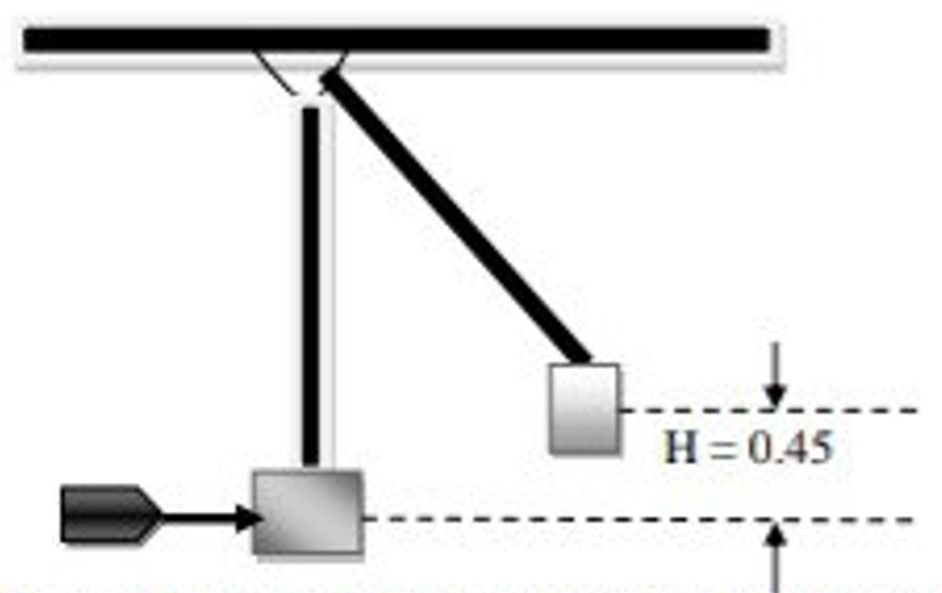
\includegraphics[scale=0.4]{Hpic.jpg}
					\end{center}
                        \begin{oneparchoices}
						\choice 303 m/s.
						\choice 300 m/s.
						\choice 90.9 m/s.
						\choice 90 m/s.
					\end{oneparchoices} 

					\question  Which one of the following statements is 
                      true about the motion of a particle in a circular 
                      path? (UUE: 2006).\\
					\begin{choices}
						\choice  The centripetal acceleration is constant if the particle's speed is constant.
						\choice The tangential acceleration can be perpendicular to the velocity vector of the particle.
						\choice The centripetal acceleration is always in the direction perpendicular to the velocity vector of the particle.
						\choice The acceleration is always perpendicular to the velocity vector of the particle.
						
					\end{choices}

					\question Two particles with masses 2$m$ and 3$m$ 
                   are moving toward each other along the $x$ axis with the 
                   same initial speeds $v$. Particle 2$m$ is traveling to 
                   the left, and particle 3$m$ is traveling to the right. 
                   They undergo an elastic glancing collision such that 
                   particle 2$m$ is moving in the negative $y$ direction 
                   after the collision. What are the $x$ component of the 
                   final velocity of particle 3$m$ and the kinetic energy of 
                   the particle 2$m$, respectively? (UEE: 2006).\\
					\begin{choices}
						\choice 0.33 $v$ and 0.7 $mv²$.
						\choice 0.33 $v$ and 1.4 $mv²$.
						\choice 0.67 $v$ and 0.7 $mv²$.
						\choice 0.67 $v$ and 1.4 $mv²$.
						
					\end{choices}
				\end{questions}
			\end{document}
